\documentclass{ximera}

\usepackage{epsfig}

\graphicspath{
  {./}
  {figures/}
}

\usepackage{epstopdf}
%\usepackage{ulem}
\usepackage[normalem]{ulem}

\epstopdfsetup{outdir=./}

\usepackage{morewrites}
\makeatletter
\newcommand\subfile[1]{%
\renewcommand{\input}[1]{}%
\begingroup\skip@preamble\otherinput{#1}\endgroup\par\vspace{\topsep}
\let\input\otherinput}
\makeatother

\newcommand{\EXER}{}
\newcommand{\includeexercises}{\EXER\directlua{dofile(kpse.find_file("exercises","lua"))}}

\newenvironment{computerExercise}{\begin{exercise}}{\end{exercise}}

%\newcounter{ccounter}
%\setcounter{ccounter}{1}
%\newcommand{\Chapter}[1]{\setcounter{chapter}{\arabic{ccounter}}\chapter{#1}\addtocounter{ccounter}{1}}

%\newcommand{\section}[1]{\section{#1}\setcounter{thm}{0}\setcounter{equation}{0}}

%\renewcommand{\theequation}{\arabic{chapter}.\arabic{section}.\arabic{equation}}
%\renewcommand{\thefigure}{\arabic{chapter}.\arabic{figure}}
%\renewcommand{\thetable}{\arabic{chapter}.\arabic{table}}

%\newcommand{\Sec}[2]{\section{#1}\markright{\arabic{ccounter}.\arabic{section}.#2}\setcounter{equation}{0}\setcounter{thm}{0}\setcounter{figure}{0}}
  
\newcommand{\Sec}[2]{\section{#1}}

\setcounter{secnumdepth}{2}
%\setcounter{secnumdepth}{1} 

%\newcounter{THM}
%\renewcommand{\theTHM}{\arabic{chapter}.\arabic{section}}

\newcommand{\trademark}{{R\!\!\!\!\!\bigcirc}}
%\newtheorem{exercise}{}

\newcommand{\dfield}{{\sf SlopeField}}

\newcommand{\pplane}{{\sf PhasePlane}}

\newcommand{\PPLANE}{{\sf PHASEPLANE}}

% BADBAD: \newcommand{\Bbb}{\bf}. % Package amsfonts Warning: Obsolete command \Bbb; \mathbb should be used instead.

\newcommand{\R}{\mbox{$\mathbb{R}$}}
\let\C\relax
\newcommand{\C}{\mbox{$\mathbb{C}$}}
\newcommand{\Z}{\mbox{$\mathbb{Z}$}}
\newcommand{\N}{\mbox{$\mathbb{N}$}}
\newcommand{\D}{\mbox{{\bf D}}}

\newcommand{\WW}{\mathcal{W}}

\usepackage{amssymb}
%\newcommand{\qed}{\hfill\mbox{\raggedright$\square$} \vspace{1ex}}
%\newcommand{\proof}{\noindent {\bf Proof:} \hspace{0.1in}}

\newcommand{\setmin}{\;\mbox{--}\;}
\newcommand{\Matlab}{{M\small{AT\-LAB}} }
\newcommand{\Matlabp}{{M\small{AT\-LAB}}}
\newcommand{\computer}{\Matlab Instructions}
\renewcommand{\computer}{M\small{ATLAB} Instructions}
\newcommand{\half}{\mbox{$\frac{1}{2}$}}
\newcommand{\compose}{\raisebox{.15ex}{\mbox{{\scriptsize$\circ$}}}}
\newcommand{\AND}{\quad\mbox{and}\quad}
\newcommand{\vect}[2]{\left(\begin{array}{c} #1_1 \\ \vdots \\
 #1_{#2}\end{array}\right)}
\newcommand{\mattwo}[4]{\left(\begin{array}{rr} #1 & #2\\ #3
&#4\end{array}\right)}
\newcommand{\mattwoc}[4]{\left(\begin{array}{cc} #1 & #2\\ #3
&#4\end{array}\right)}
\newcommand{\vectwo}[2]{\left(\begin{array}{r} #1 \\ #2\end{array}\right)}
\newcommand{\vectwoc}[2]{\left(\begin{array}{c} #1 \\ #2\end{array}\right)}

\newcommand{\ignore}[1]{}


\newcommand{\inv}{^{-1}}
\newcommand{\CC}{{\cal C}}
\newcommand{\CCone}{\CC^1}
\newcommand{\Span}{{\rm span}}
\newcommand{\rank}{{\rm rank}}
\newcommand{\trace}{{\rm tr}}
\newcommand{\RE}{{\rm Re}}
\newcommand{\IM}{{\rm Im}}
\newcommand{\nulls}{{\rm null\;space}}

\newcommand{\dps}{\displaystyle}
\newcommand{\arraystart}{\renewcommand{\arraystretch}{1.8}}
\newcommand{\arrayfinish}{\renewcommand{\arraystretch}{1.2}}
\newcommand{\Start}[1]{\vspace{0.08in}\noindent {\bf Section~\ref{#1}}}
\newcommand{\exer}[1]{\noindent {\bf \ref{#1}}}
\newcommand{\ans}{\textbf{Answer:} }
\newcommand{\matthree}[9]{\left(\begin{array}{rrr} #1 & #2 & #3 \\ #4 & #5 & #6
\\ #7 & #8 & #9\end{array}\right)}
\newcommand{\cvectwo}[2]{\left(\begin{array}{c} #1 \\ #2\end{array}\right)}
\newcommand{\cmatthree}[9]{\left(\begin{array}{ccc} #1 & #2 & #3 \\ #4 & #5 &
#6 \\ #7 & #8 & #9\end{array}\right)}
\newcommand{\vecthree}[3]{\left(\begin{array}{r} #1 \\ #2 \\
#3\end{array}\right)}
\newcommand{\cvecthree}[3]{\left(\begin{array}{c} #1 \\ #2 \\
#3\end{array}\right)}
\newcommand{\cmattwo}[4]{\left(\begin{array}{cc} #1 & #2\\ #3
&#4\end{array}\right)}

\newcommand{\Matrix}[1]{\ensuremath{\left(\begin{array}{rrrrrrrrrrrrrrrrrr} #1 \end{array}\right)}}

\newcommand{\Matrixc}[1]{\ensuremath{\left(\begin{array}{cccccccccccc} #1 \end{array}\right)}}



\renewcommand{\labelenumi}{\theenumi}
\newenvironment{enumeratea}%
{\begingroup
 \renewcommand{\theenumi}{\alph{enumi}}
 \renewcommand{\labelenumi}{(\theenumi)}
 \begin{enumerate}}
 {\end{enumerate}
 \endgroup}

\newcounter{help}
\renewcommand{\thehelp}{\thesection.\arabic{equation}}

%\newenvironment{equation*}%
%{\renewcommand\endequation{\eqno (\theequation)* $$}%
%   \begin{equation}}%
%   {\end{equation}\renewcommand\endequation{\eqno \@eqnnum
%$$\global\@ignoretrue}}

%\input{psfig.tex}

\author{Martin Golubitsky and Michael Dellnitz}

%\newenvironment{matlabEquation}%
%{\renewcommand\endequation{\eqno (\theequation*) $$}%
%   \begin{equation}}%
%   {\end{equation}\renewcommand\endequation{\eqno \@eqnnum
% $$\global\@ignoretrue}}

\newcommand{\soln}{\textbf{Solution:} }
\newcommand{\exercap}[1]{\centerline{Figure~\ref{#1}}}
\newcommand{\exercaptwo}[1]{\centerline{Figure~\ref{#1}a\hspace{2.1in}
Figure~\ref{#1}b}}
\newcommand{\exercapthree}[1]{\centerline{Figure~\ref{#1}a\hspace{1.2in}
Figure~\ref{#1}b\hspace{1.2in}Figure~\ref{#1}c}}
\newcommand{\para}{\hspace{0.4in}}

\usepackage{ifluatex}
\ifluatex
\ifcsname displaysolutions\endcsname%
\else
\renewenvironment{solution}{\suppress}{\endsuppress}
\fi
\else
\renewenvironment{solution}{}{}
\fi

\ifcsname answer\endcsname
\renewcommand{\answer}{}
\fi

%\ifxake
%\newenvironment{matlabEquation}{\begin{equation}}{\end{equation}}
%\else
\newenvironment{matlabEquation}%
{\let\oldtheequation\theequation\renewcommand{\theequation}{\oldtheequation*}\begin{equation}}%
  {\end{equation}\let\theequation\oldtheequation}
%\fi

\makeatother

\newcommand{\RED}[1]{{\color{red}{#1}}} 


\title{MATLAB ODE}

\begin{document}
\begin{abstract}
\end{abstract}
\maketitle

\label{S:ode45}

Previously, we have used {\dfield}, {\sf pline}, and {\pplane}
to compute solutions to one and two dimensional ordinary differential
equations numerically.  We now wish to compute solutions to higher dimensional
systems of ordinary differential equations and to do this we will use the 
\Matlab command {\tt ode45}.\index{\computer!ode45}  \Matlab provides the 
command {\tt ode45}, among others, for solving initial value problems, and we 
illustrate how this command works on several examples.  In this section we 
illustrate the command on a simple one dimensional example and in the next
section we will compute solutions to three and four dimensional systems.

\subsubsection*{A Simple One Dimensional Example}

Suppose that we want to compute numerically the solution of the initial value 
problem\index{initial value problem}
\arraystart
\begin{equation}   \label{eq:fexam}
\begin{array}{rcl}
\dps \frac{dx}{dt}(t) & = & x(t)+t \\
x(t_0) & = & x_0
\end{array}
\end{equation}
\arrayfinish
on the time interval $t\in [t_0,t_e]$.  Then the {\em data\/} of this 
problem are 
\begin{itemize}
\item the numbers $x_0,t_0$ and $t_e$, and 
\item the function $f(t,x)=x+t$.  
\end{itemize}
We know how to assign specific values for $t_0,x_0$ and $t_e$ in \Matlabp;
we will call these variables {\tt t0, x0} and {\tt te}.  Before proceeding, 
we need to understand how to make a function $f(t,x)$ available for 
computations in \Matlabp.

\subsection*{The Construction of m-files in MATLAB}\index{\computer!m-file}

Functions that are used by \Matlab are defined via 
{\em m-files}.  We now show how to construct m-files with two examples.

Suppose that we want the function $g:\R^2\to\R$, defined by
\begin{matlabEquation}  \label{eq:gexam}
g(y,z) = yz^2 + \sin y,
\end{matlabEquation}
to be available in \Matlabp.
Then we specify $g$ by writing a \Matlab m-file that contains the information 
defining this function.  The m-file {\tt gexam.m} that defines the function 
$g(y,z)$ in \eqref{eq:gexam} has two lines:
\begin{verbatim}
function g = gexam(y,z)
g = y*z^2 + sin(y);
\end{verbatim}\index{\computer!function}
The first line states that 
\begin{itemize}
\item this m-file contains a {\tt function} with the name {\tt gexam},
\item the input arguments are {\tt y} and {\tt z}, and
\item the output variable is {\tt g}.
\end{itemize}
The value of the function $g$ at the point ${\tt (y,z)}$ is given in the 
second line 
\begin{verbatim}
g = ... ;   
\end{verbatim}
Note that this line must end with a semicolon. 
\begin{quote}
{\bf Remark:} When \Matlab is used under Windows or on a PowerMac, then 
m-files
can be created using the {\sf New} entry in the {\sf File} menu.
On Unix based systems we must create the m-file using a separate
editor.  In any case make sure that the new m-file is stored in the directory
where \Matlab has been started.
\end{quote}
As an exercise, create the m-file {\tt gexam.m}.  The function $g$ is 
now available in \Matlabp; when we type {\tt gexam(1,2)}, 
we obtain the answer \verb+4.8415+, which is indeed $g(1,2)=4+\sin(1)$.

We store function m-files with the other {\sf laode} files using the prefix
{\tt f} (for function) followed by the equation number.  So the m-file 
{\tt gexam.m} is stored as {\tt f14\_3\_2.m}.  Indeed, compare the result of 
typing {\tt f14\_3\_2(1,2)} with {\tt gexam(1,2)}.

Both the input arguments and the output variable in an m-file can consist of 
vectors\index{vector}.  For instance, suppose that we want to define the function 
$h:\R^3\to\R^2$ where $u=(u_1,u_2,u_3)^t\in\R^3$ and  
\begin{matlabEquation}\label{MATLAB:42}
h(u) = \left(\begin{array}{c} u_1 u_2\\ u_2-u_1 u_3 \end{array}\right).
\end{matlabEquation}
As a second exercise, write the m-file\index{\computer!m-file} {\tt hexam.m} 
as follows:
\begin{verbatim}
function h = hexam(u)
h = [u(1)*u(2), u(2)-u(1)*u(3)]';
\end{verbatim}
The command {\tt w = hexam([1,2,3])} gives the answer
\begin{verbatim}
w =
     2
    -1
\end{verbatim}
which is indeed $h(1,2,3)$.  This m-file has been stored as {\tt f14\_3\_3.m}.

\subsection*{The \Matlab Command {\tt ode45}}\index{\computer!ode45}

We now return to the initial value problem \eqref{eq:fexam}.
The function 
\begin{matlabEquation}\label{MATLAB:43}
f(t,x)=x+t
\end{matlabEquation}
on the right hand side is available to \Matlab in the m-file 
{\tt f14\_3\_4.m}, which is stored with the other {\sf laode\/} files: 
\begin{verbatim}
function f = f14_3_4(t,x)
f = x + t;
\end{verbatim}

The \Matlab command 
\begin{center}
{\tt ode45('f14\_3\_4',[t0 te],x0)}
\end{center}\index{\computer!ode45} 
computes a numerical approximation to the solution to the initial value 
problem \eqref{eq:fexam} on the interval {\tt [t0,te]}.
For instance, we can use {\tt ode45} to solve the initial value problem
\begin{equation}  \label{eq:fexam1}
\begin{array}{rcl}
\dps \frac{dx}{dt} & = & x+t \\
x(1) & = & 2
\end{array}
\end{equation}
for $t\in[1,3]$. In this case, $t_0=1$, $t_e=3$, and $x_0=2$.  After 
typing the command
\begin{verbatim}
[t,x] = ode45('f14_3_4',[1 3],2);
\end{verbatim}
the approximate solution is stored in the vectors {\tt t} and {\tt x}.
The components of the vector {\tt t} are the values of $t$ for which the 
solution has been computed, and the components of the vector {\tt x} are 
the values of the solution $x$ at the values {\tt t}.  Indeed, typing 
{\tt t} and {\tt x} we see that both vectors have length $45$.   The
length of the vectors {\tt t} and {\tt x} is chosen by {\tt ode45} so
as to guarantee a certain accuracy in the solution.  We discuss this 
issue in greater detail below.

We can visualize the solution by plotting its time series\index{time series}:
\begin{verbatim}
plot(t,x)
xlabel('t')
ylabel('x')
\end{verbatim}\index{\computer!plot}
The result is shown in Figure~\ref{fig:ode45ex1}.  

\begin{figure}[htb]
   \centerline{%
   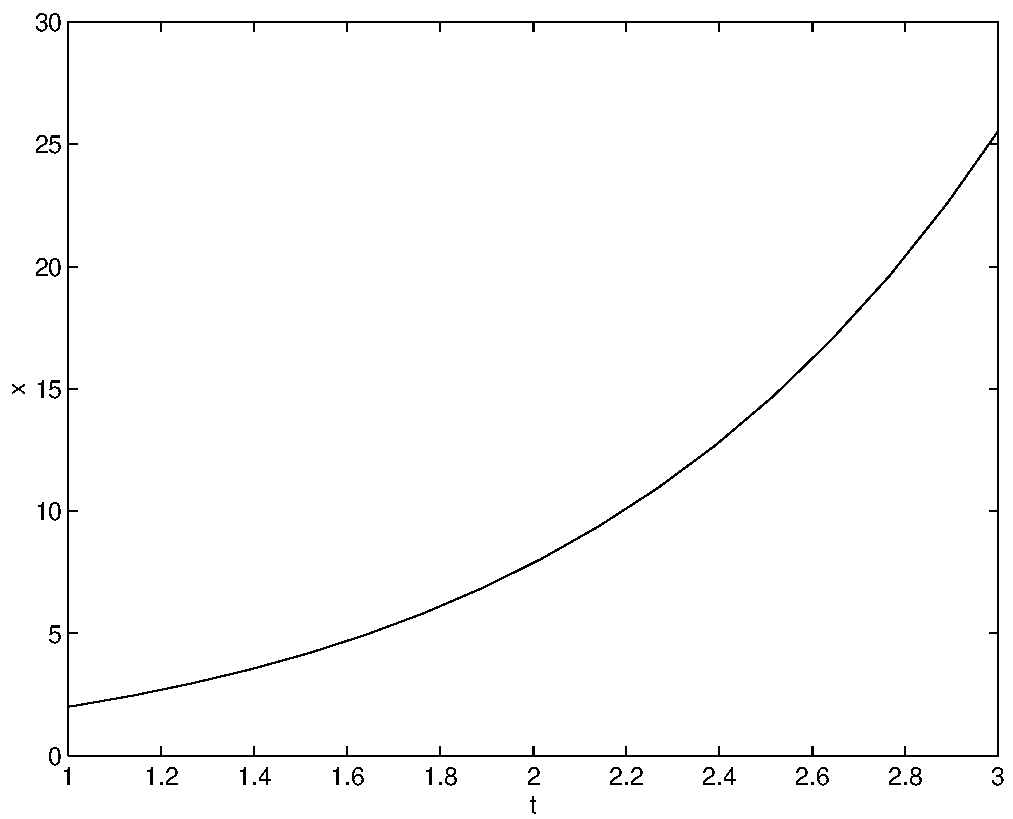
\includegraphics[width=3.2in]{../figures/ode45ex1.pdf}}
   \caption{Approximation of the solution of
   \protect\eqref{eq:fexam1} obtained by {\tt ode45} in \protect\Matlabp.}
   \label{fig:ode45ex1}
\end{figure}

In fact, the initial value problem \eqref{eq:fexam1} has a simple closed form 
solution
\[
x(t) = 4e^{t-1}-t-1,
\]
which can be verified directly by differentiation.  The existence of this
closed form solution allows us to check the accuracy of the numerical
calculations made by {\tt ode45}.  Indeed, graphically we cannot distinguish 
the result obtained using {\tt ode45}\index{\computer!ode45} from the exact 
solution.  To verify this point, type
\begin{verbatim}
x_exact = 4*exp(t-1)-t-1;
hold on
plot(t,x_exact,'r')
\end{verbatim}
and observe that the graph of the exact solution, which is in red, exactly
covers the plot of the numerically computed solution.

\subsection*{Accuracy of {\tt ode45}}
\index{accuracy of {\tt ode45}}

We now discuss the error made by {\tt ode45} in more detail.
\index{\computer!ode45}
Using {\tt ode45} we obtained an approximation of the solution of
the initial value problem \eqref{eq:fexam1} at the times $t_k={\tt t(k)}$
for $k=1,2,\ldots,45$.  The exact solution at these points is
\[
x(t_k)=4e^{t_k-1}-t_k-1,
\]
and the {\tt ode45} approximation to the solution is $x_k={\tt x(k)}$.  The 
routine {\tt ode45} automatically computes the solution subject to satisfying 
two constraints: {\em absolute error} and {\em relative error\/}.

The {\em absolute error}\index{error!absolute} is just the absolute value of
the difference between the numerically computed solution and the exact
solution, that is,
\[
\epsilon_{abs}(k) = |x_k - x(t_k)|.
\]
We can visualize the absolute error by plotting $\epsilon_{abs}$ versus $t$, 
as follows:
\begin{verbatim}
err_abs = abs(x-x_exact);
plot(t,err_abs)
xlabel('t')
ylabel('absolute error')
\end{verbatim}
The \Matlab command {\tt abs(v)} generates a vector containing the absolute 
values of the components of the vector {\tt v}.  The result is presented in 
Figure~\ref{fig:ode45err0}.  Note that even though the absolute error 
oscillates, it is always less than $6\cdot10^{-6}$, which is why we could not 
distinguish the graph of the exact solution from the graph of the numerically 
computed solution given in Figure~\ref{fig:ode45ex1}.

\begin{figure}[htb]
   \centerline{%
   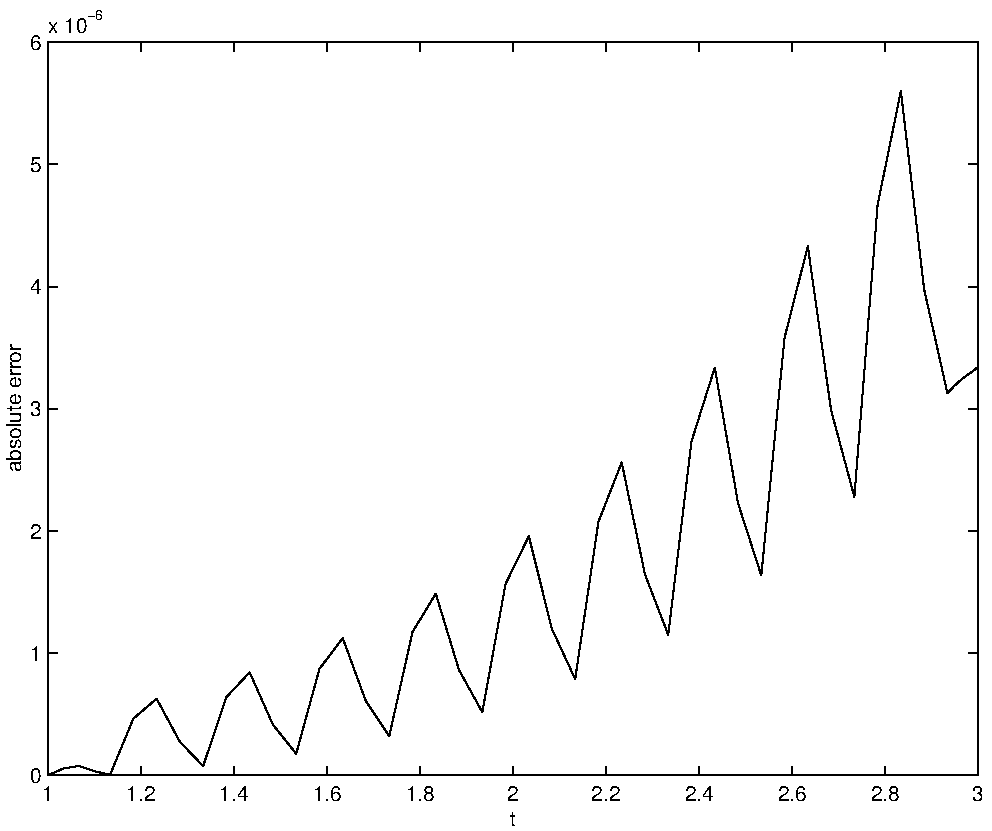
\includegraphics[width=3.2in]{../figures/ode45err0.pdf}}
   \caption{Absolute error in the approximation of the solution of
   \protect\eqref{eq:fexam1} obtained by {\tt ode45} in \protect\Matlab with 
	default error bound {\tt 1e-6}.}
   \label{fig:ode45err0}
\end{figure}

Having an absolute error of $10^{-6}$ in a numerically computed solution might
seem quite good --- unless we happened to be computing a solution whose size 
is $10^{-7}$.  Then the numerical error would be ten times the size of the 
solution itself, which is a huge error.  For this reason, numerical analysts
like to use another measure for success.  

The {\em relative error\/}\index{error!relative} between 
the approximation and the exact solution is the absolute error normalized by 
the size of the exact solution, that is  
\[
\epsilon_{rel}(k) = \frac{\epsilon_{abs}(k)}{|x(t_k)|} 
= \frac{|x_k - x(t_k)|}{|x(t_k)|}.
\]
The numbers $\epsilon_{rel}(k)$ must be uniformly small in order to guarantee
a good numerical approximation to the actual solution.  Using the fact
that we have a formula for the exact solution, we can compute the numbers 
$\epsilon_{rel}$ and plot them in \Matlab by typing
\begin{verbatim}
err_rel = abs(x-x_exact)./abs(x_exact);
plot(t,err_rel)
xlabel('t')
ylabel('relative error')
\end{verbatim} 
The result is shown in Figure~\ref{fig:ode45err1}.  We see that the relative 
error oscillates, but is always smaller than $3\cdot 10^{-7}$.
\begin{figure}[htb]
   \centerline{%
   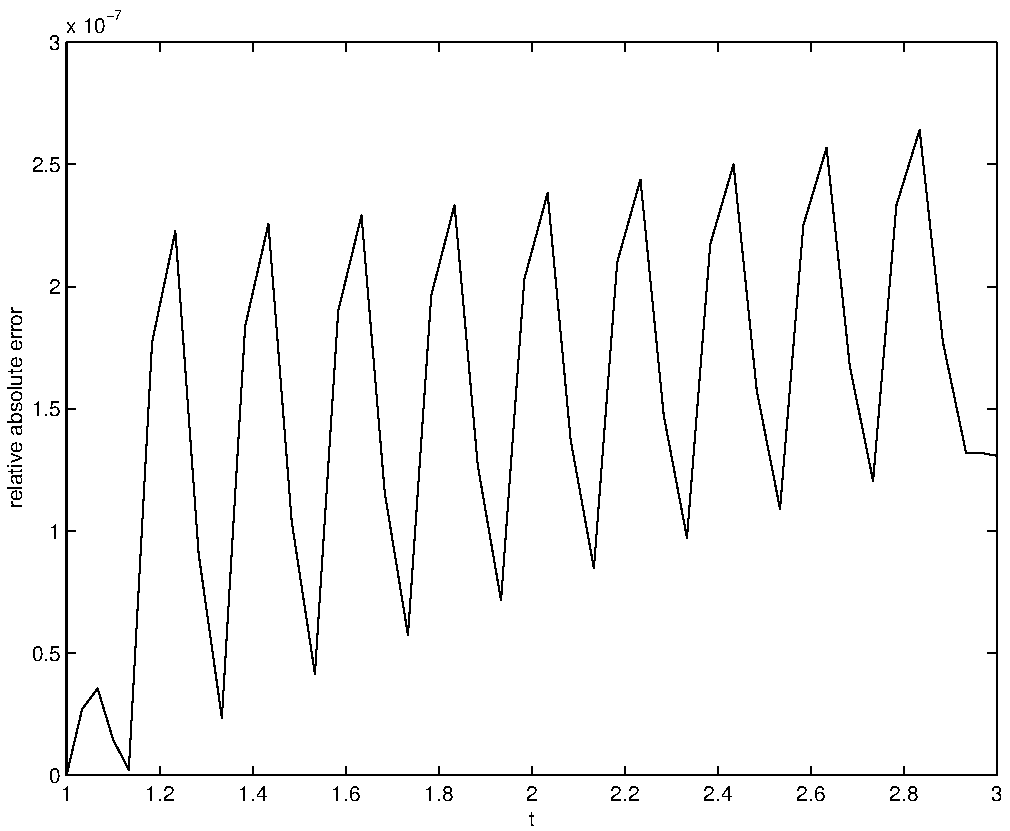
\includegraphics[width=3.2in]{../figures/ode45err1.pdf}}
   \caption{Relative error in the approximation of the solution of
   \protect\eqref{eq:fexam1} obtained by {\tt ode45} in \protect\Matlab with 
	default error bound {\tt 1e-3}.}
   \label{fig:ode45err1}
\end{figure}

Default error bounds are preset in the command {\tt ode45}.  Unless otherwise
instructed {\tt ode45} {\em attempts\/} to find a numerical approximation 
whose absolute error is everywhere less than $10^{-6}$ and whose relative 
error is everywhere less than $10^{-3}$.  (There is a interesting mathematical
question concerning how these bounds are actually satisfied, since 
{\tt ode45} does not, in fact, know the exact solution.)  We can use 
{\tt ode45} to compute an approximation of the solution with an even smaller 
error.  To set this smaller error, we add an argument to the call of 
{\tt ode45} by typing 
\begin{verbatim}
options = odeset('RelTol',1e-8);
[t,x]=ode45('f14_3_4',[1 3],2,options);
\end{verbatim}
These instructions compute an approximation for which the relative error 
\index{error!relative} is smaller than $10^{-8}$.  
(Type {\tt odeset}\index{\computer!odeset} in \Matlab in order to see a 
complete list of options. Type {\tt options} to see a list of the currently
specified options.)  Hence, when we perform 
this calculation, we expect to obtain an even better result than before.  
Indeed, proceeding as above, we obtain the relative error shown 
in Figure~\ref{fig:ode45err2}.  In an attempt to guarantee the reduced error, 
{\tt ode45} generates 61 time steps during the computation.  

\begin{figure}[htb]
   \centerline{%
   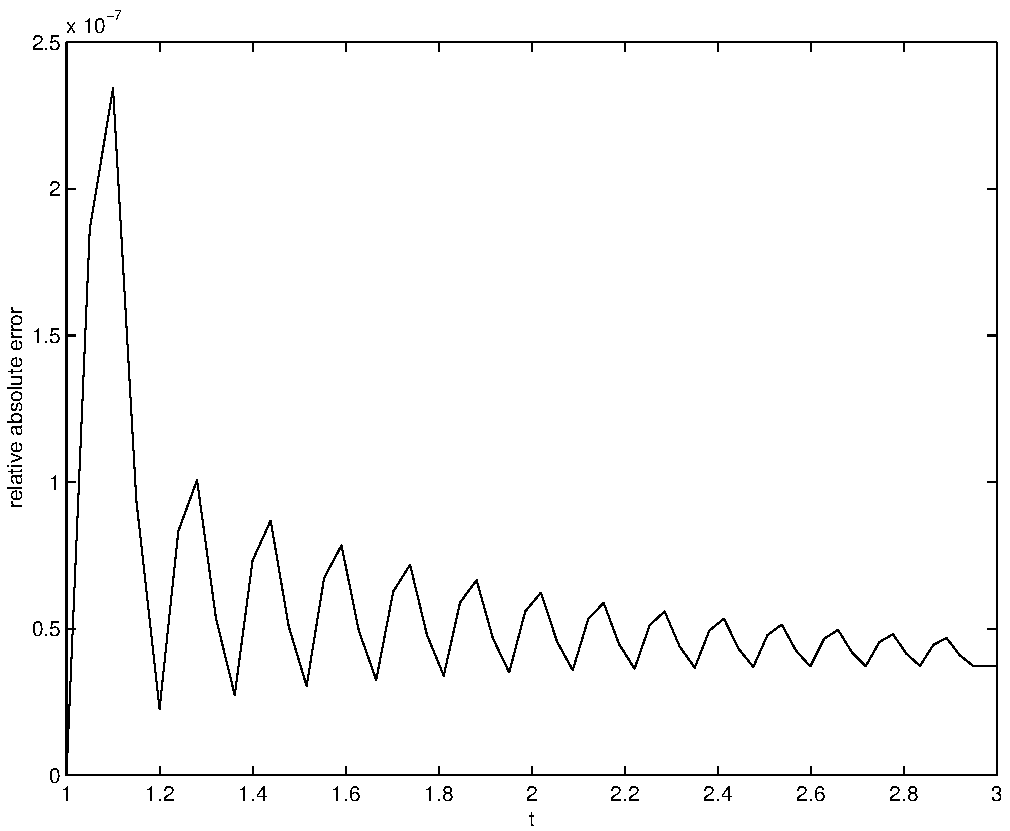
\includegraphics[width=3.2in]{../figures/ode45err2.pdf}}
   \caption{Relative error in the approximation of the solution of
   \protect\eqref{eq:fexam1} obtained by {\tt ode45} in \protect\Matlab with 
	{\tt 1e-8} error bound.}
   \label{fig:ode45err2}
\end{figure}



\includeexercises



\end{document}
